\documentclass[10pt]{article}
\usepackage[margin=1in]{geometry}
\usepackage[shortlabels]{enumitem}
%\setcounter{secnumdepth}{0}
\usepackage{amssymb,amsmath,amsthm}
\usepackage{graphicx}
\usepackage{caption}
\usepackage{fancyhdr, lastpage}
\pagestyle{fancy}
\fancyhf{}
\lhead{Daniel Standage}
\chead{GDCB 511, 9:00am MWF}
\rhead{Lecture Notes: 10-15 Feb, 2012}
%\cfoot{Page \thepage{} of \protect\pageref*{LastPage}}
\usepackage{varioref}
\labelformat{equation}{(#1)}
\usepackage[colorlinks,linkcolor=blue]{hyperref}

\newenvironment{mitemize}
{
  \begin{itemize}
  \setlength{\itemsep}{1pt}
  \setlength{\parskip}{0pt}
  \setlength{\parsep}{0pt}}{\end{itemize}
}

\newenvironment{menumerate}
{
  \begin{enumerate}
  \setlength{\itemsep}{1pt}
  \setlength{\parskip}{0pt}
  \setlength{\parsep}{0pt}}{\end{enumerate}
}

\newcommand{\textsup}[1]{\ensuremath{^{\textrm{#1}}}}
\newcommand{\textsub}[1]{\ensuremath{_{\textrm{#1}}}}


\begin{document}

\section*{Combinatorial code}
\begin{mitemize}
  \item Different combinations of transcription activators (and/or other cofactors) produce different evels of expression of a given gene or set of genes in different cellular, development, or environmental conditions.
  \item Combinatorial controls ensure a gene or set of genes are tunred on at the right time and right place to perform specific functions, or specify certain cell/tissue/organ types.
  \item Formation of enhanceosome is one way to implement combinatorial control.
\end{mitemize}

\section*{Insulators}
\begin{mitemize}
  \item DNA elements that can shield genes from activation or repression
  \item two functional hypotheses: sliding model (block enhancers/silencers), looping model (dimers form loops to isolate enhancers/silencers from promoter)
  \item two or more insulators can cancel or enhance each other's effects
\end{mitemize}
\vspace{25px}

\begin{center}
  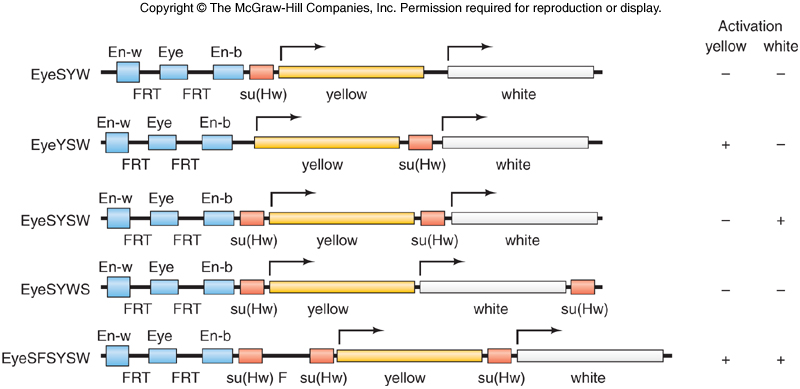
\includegraphics{insulators.jpg}
\end{center}

\section*{Regulation of transcription factors}
Signal transduction pathways can modify transrciption factors, regulating their activity.
\begin{mitemize}
  \item phosphorylation
  \item ubiquitination
  \item acetylation
  \item methylation
  \item others
\end{mitemize}

\subsection*{Example: p53 tumor suppressor protein}
\begin{mitemize}
  \item atypical binding domain
  \item promotes growth arrest, apoptosis, and cell senescence
  \item regulates many genes
  \item regulated by many genes
\end{mitemize}
\vspace{25px}

\begin{center}
  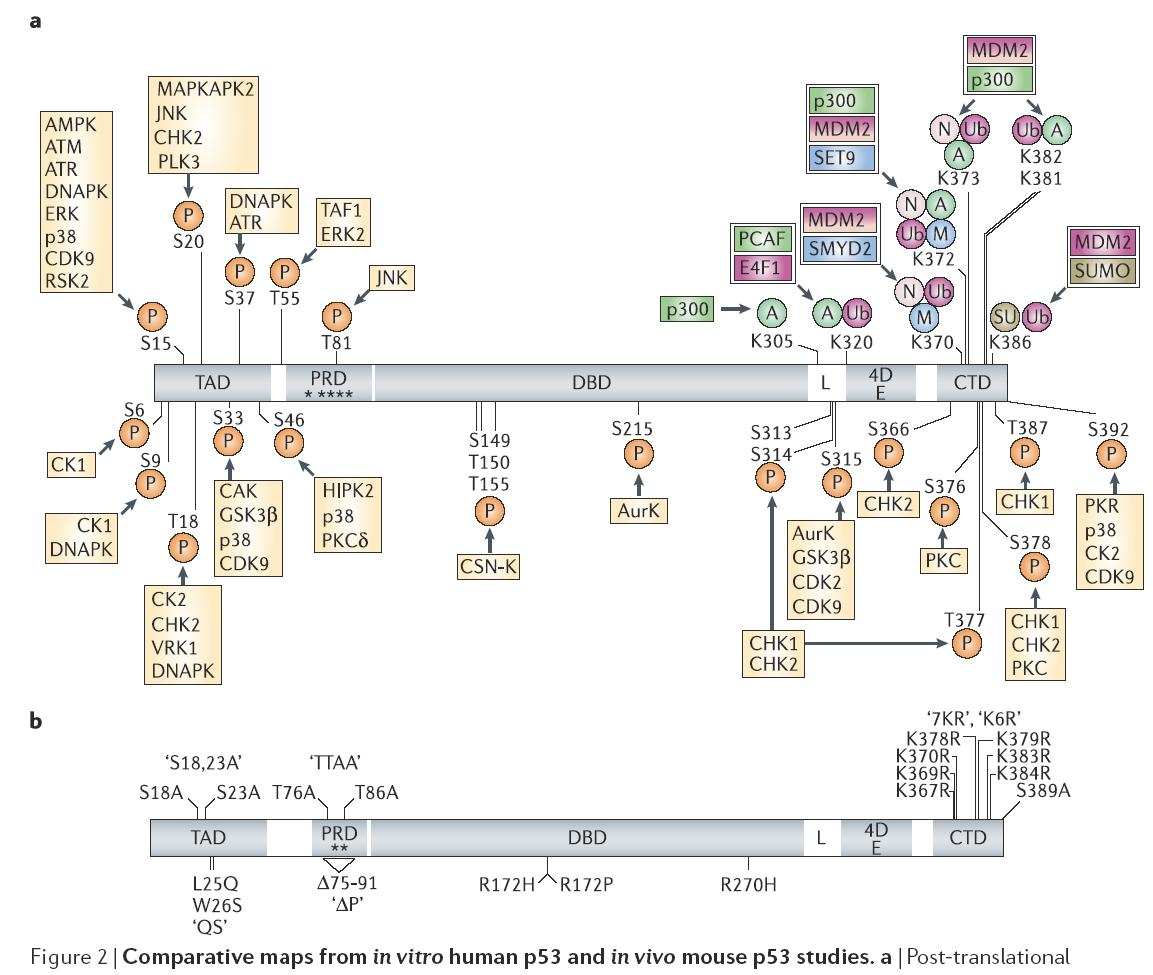
\includegraphics[width=450px]{p53mods.jpg}
\end{center}

\subsubsection*{Acetylation}
\begin{itemize}
  \item acetylation of p53 (in C terminal domain) enhances DNA binding activity
  \item p53 is fully acetylated on DNA damage and correlates with expression of p53 target genes (p21 particularly)
\end{itemize}

\subsubsection*{Phosphorylation}
\begin{itemize}
  \item HIPK2 is activated by UV radiation and phosphorylates p53
  \item p53 acetylation (by CBP/p300) is dependent on phosphorylation by HIPK2
  \item enhances expression of p53 gene targets (esp. p21)
  \item HIPK2 inhibits cell proliferation, results in growth arrest and apoptosis
\end{itemize}

\subsubsection*{Ubiquitination}
\begin{itemize}
  \item MDM2 does not affect p53 mRNA
  \item MDM2 causes a reduction of p53
  \item MDM2 ubiquitinates p53
  \item USP10 stabilizes and deubiquitinates p53, promotes p53 activity
  \item MDM2 moves p53 to cytoplasm by ubiquitination
  \item USP10 deubiquitinates p53
  \item under unstressed conditions, MDM2 succeeds and p53 is degraded; under genotoxic stress conditions, USP10 succeeds and p53 gene targets are expressed, apoptosis elicited
\end{itemize}

\subsubsection*{Methylation}
\begin{itemize}
  \item Set9 has specificay methyltransferase activity, specific to p53 and H3
  \item p53 is not methylated by many common methyltransferases
  \item Set9 methylates p53 at K372
  \item Set9 enhances expression of p53 target genes
  \item Smyd2 methylates p53 at K370
  \item Smyd2 represses p53 function
  \item crosstalk between Set9 and Smyd9; methylation of K370 has no affect on methylation of K372, but methylation of K372 shuts down methylation of K370
\end{itemize}

\end{document}
